\section{Blind Test Accorshotel Arena}

\subsection{AccorHotels Arena}

Accorhotel est le premier gerant d'hotel de france et le 6e mondial.
A l'occasion d'un partenariat, le Palais omnisports de Paris-Bercy c'est vu renommé AccorHotel Arena pour 10 ans.

Le site acceuillant beaucoup de concerts et de spectateurs, accorshotel a voulu communiquer au travers d'une installation interactive.
Cette installation est un blind test composé d'un ecran et d'un Ipad permettant de saisir les réponses.

Le jeu est simple : Une chanson est jouée sur l'écran et le titre de cette chanson est indiqué.
Le joueur dispose alors de 45 secondes pour trouver l'artiste en question parmi les 4 proposés.
On enchaîne ainsi sur 6 questions qui se terminent sur le résultat du jeu affiché à l'utilisateur.e installation permettant de jouer à un Blind Test sur un écran.

\subsection{Technologies}

Les technologies utilisées dans ce projet sont standards et étaient déjà maîtrisées par les membres de l'équipe.
On retrouve alors une application \emph{Electron} pour l'affichage sur l'écran et un serveur NodeJS avec le framework \emph{Express} pour servir les fichiers et gérer le jeu.
Enfin, on utilise \emph{Socket.io} pour les WebSocket apportant de l'interactivité.

\subsubsection{Express}

Express est une librairie utilisant les capacités de NodeJs (inclus dans electron) à mettre en place un serveur web.
Express permet de répondre à une URL mais aussi de servir des fichiers en tout genre.

Nous avons choisis express car il est légé et simple à mettre en place.
Il dispose d'une grande communauté et permet de mettre en place un serveur web et websocket rapidement.

Nous n'avions pas besoin ici d'une solution plus lourde car les seuls interactions HTTP sont les demandes de médias comme la musique et les images ou la demande de page WEB.
Le reste des interactions s'éfféctuent au travers des Websockets.

\subsubsection{WebSockets}

La technologie de Websocket est un protocol web de connexion bidirectionnel semblables aux sockets.
Ils permettent au serveur et au client de conserver une connexion TCP bidirectionnel.

Ainsi il est possible au client d'envoyer des paquets arbitraires au serveur mais aussi, et c'est le plus interessant, au serveur d'envoyer des paquets au client a n'importe quel moment.
Ainsi, il est possible de rendre l'application tres interactive et dynamique.

Nous avons utilisé les WebSockets pour toute la communication entre le serveur et les clients (Ecran et Ipad) avec l'aide de Socket.io.
Cette librairie se place comme une surcouche aux websocket et reprend l'aspect évenementiel de Nodejs.
En effet, elle met a disposition du developpeur un objet \texttt{socket} agissant comme un emetteur et un recepteur d'évenements.
chaque évenement est composé d'un nom et d'un objet de contexte.
Lors de l'émission, l'objet \texttt{socket} transmet l'évenement et le contexte au client connecté.
Il est aussi possible de recevoir des évenements et ainsi de communiquer de manière bidirectionnel.

\subsection{Structure}

Le Blind Test se compose de 3 éléments.

\paragraph{Le serveur Web} présent dans le processus principal de l'application Electron, il gère tout le jeu du début à la fin.
Il présente un serveur de fichiers permettant l'accès aux fichiers audio, aux fichiers d'image et aux pages Web depuis l'iPad et l'affichage.
Il dispose aussi d'un serveur WebSockets permettant une communication bidirectionnelle entre les clients (iPad et TV) et le serveur.

Ce serveur Web dispose d'un état définissant l'état actuel du jeu.
Cet état est transmis à tous les clients pour qu'ils actualisent leur affichaient lors d'un changement et de la connexion d'un nouveau client.

Le serveur Web construit en parallèle un objet Javascript \texttt{Game} contenant toutes les questions à poser, la question actuellement posée, les réponses des joueurs et le score.
Cet objet \texttt{Game} est transmis à chaque client lors de leur connexion ou lors du changement d'état du jeu.

Des que l'etat du jeu change, un evenement socket.io est transmis à tout les clients connectés pour qu'ils actualisent leur affichage en fonction des données transmises par le serveur.

\paragraph{Les clients (TV et iPad)} Chacun charge une page HTML spécifique possédant un script spécifique.
Ce script va afficher le bon écran en fonction de l'état du jeu envoyé par le serveur et, éventuellement, demander une interaction à l'utilisateur.

Dès qu'un joueur tape sur une réponse, l'iPad envoie à son tour un paquet WebSocket au serveur pour qu'il l'enregistre et change d'état.
Le jeu continue alors jusqu'a ce que toutes les questions de tous les joueurs soient posées.

\begin{figure}[h]
    \centering
    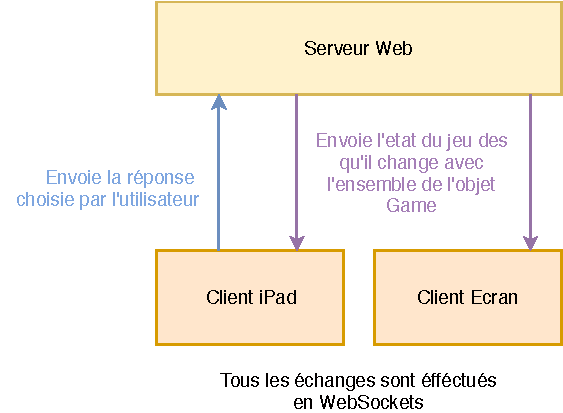
\includegraphics{img/ah-blindtest.pdf}
    \caption{Structure du jeu Blind Test}
\end{figure}

\subparagraph{TV} Coté TV, l'affichage est simple et permet d'afficher le score de l'utilisateur ainsi que de jouer la musique.
L'ecran n'etant pas tactile, il ne permet que l'affichage d'informations sur l'etat du jeu mais aucune interactivité n'est possible directement.
Le client TV est une fenêtre de l'application Electron qui se connecte au sereveur express pour y charger l'interface.

\subparagraph{Ipad} Coté Ipad, une application de kiosk permet d'afficher une page Web sans autre élément d'interface.
Cette page Web est chargée depuis le serveur et propose des choix a l'utilisateur en fonction de l'etat du jeu.
Cela peut être le nombre de joueurs, le nom de l'artiste en cours de lecture ou simplement une demande pour passer à la question suivante.

\subsubsection{Design}

Le design de l'application était fourni avec la demande du client et nous avons juste intégré ce design en extrayant des images clés du fichier Photoshop du designer.

\begin{figure}[h]
    \centering
    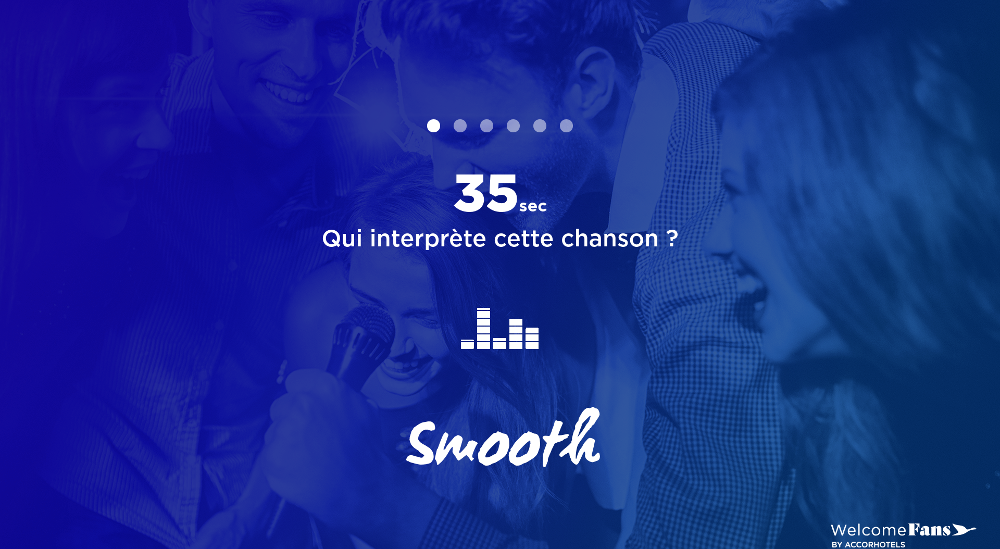
\includegraphics[scale=0.23]{img/blind-test-tv.png}
    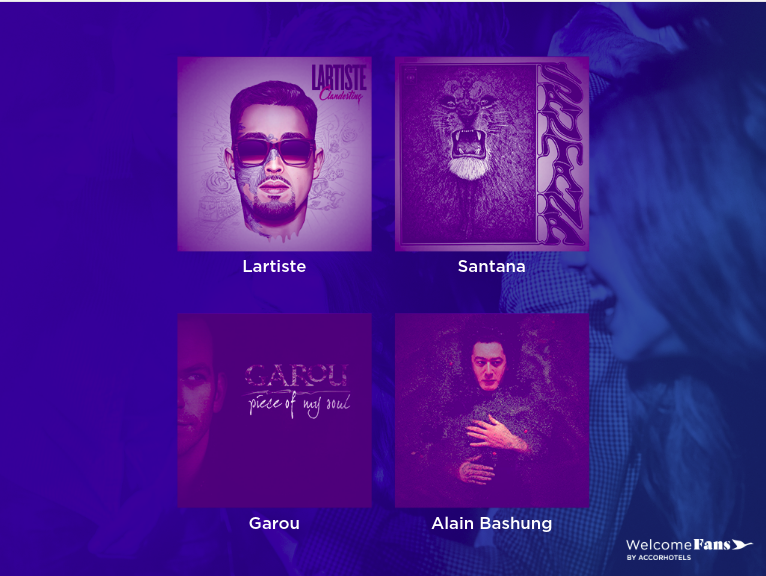
\includegraphics[scale=0.22]{img/blind-test-ipad.png}
    \caption{Une vue du Blind Test côté TV (à gauche) et côté iPad (à droite)}
\end{figure}

\subsubsection{Installation}

Je n'ai pas pu assister à l'installation du lundi 29 janvier mais j'ai tout de même travailler dessus a l'occasion de correctionde bugs.

L'installation présente un grand écran connecté au serveur affichant l'interface TV sur uen machine Windows herbergeant le serveur websocket que l'Ipad pourras contacter.
On y retrouve bien evidemment L'Ipad vérouillé pour éviter de sortir de l'application.
Ces deux terminaux sont connectés à une même borne Wifi permettant de disposer de son propre réseau évitant ainsi les latances dues a une éventuelle surcharge du réseau environnant.
Cette borne Wifi fait office de routeur vers l'exterieur mais aussi de serveur DHCP et de point d'acces Wifi.

\begin{figure}[h]
    \centering
    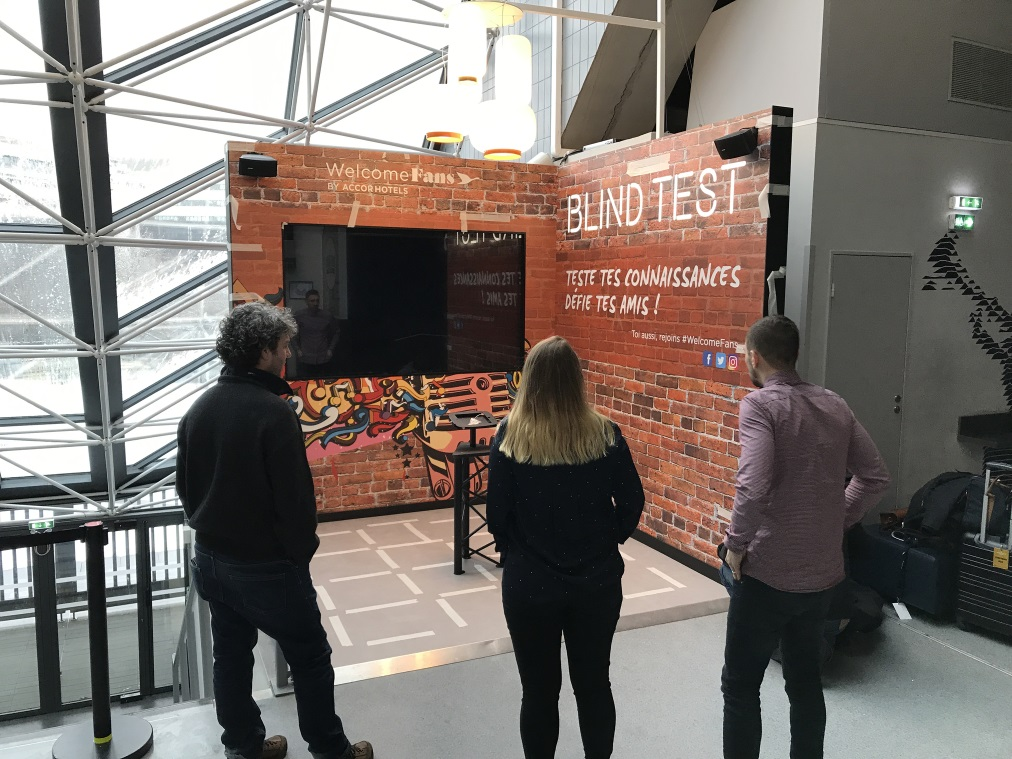
\includegraphics[scale=0.1]{img/accorhotel-blindtest-resize.jpg}
    \caption{Installation du Blind test au AccorHotel Arena}
\end{figure}

\subsubsection{Conclusion}

Ce projet fut intéressant et intense, car nous l'avons réalisé en seulement 2 jours.
Ce fut une bonne expérience de travail d'équipe et m'a permis de tester un projet à court délai.
Enfin, ce projet m'a permis de voir les techniques permettant de synchroniser l'etats de multiples machines au travers de Websocket.